\chapter{Conclusion}\label{ch:conclusion}
To sum up, this PhD work use Mixed reality game - AtomicOrchid as a testbed to probe the design issues and implications for agent planning support system. Field trials were conducted for three versions of AtomicOrchid game with different interaction design patterns (Figure \ref{fig:connections}). The first prototype is a non agent version of the game. The second and third studies are designed to probe two interaction design patterns (On-the-loop and In-the-loop). Video and system logs of the field trials are collected and interaction analysis is conducted to generate design requirements and interaction design implications. \\

\begin{figure}[H]
  \centering
  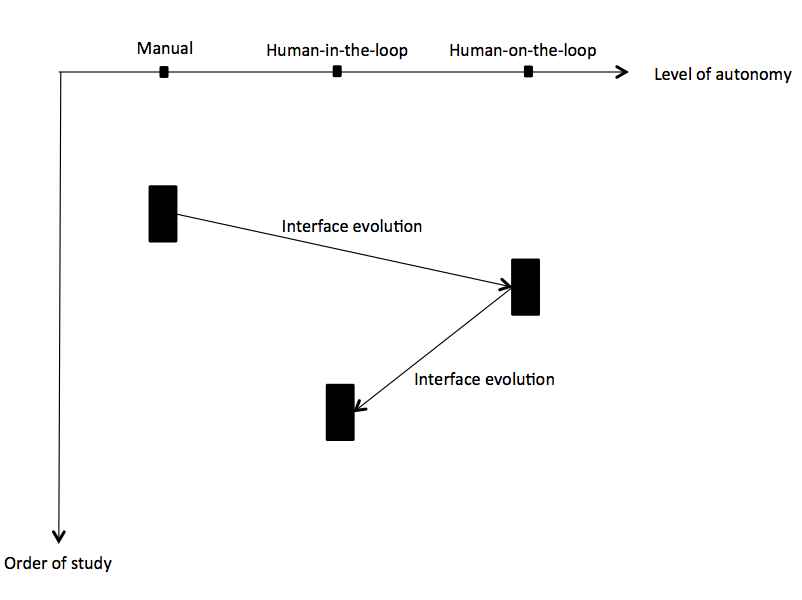
\includegraphics[width=1\textwidth]{img/conclusion/studies}
  \caption{Overview of studies}
  \label{fig:connections}
\end{figure}

The following sections summarise the contributions of the thesis, and concludes the thesis with limitations and an outlook on future work that this thesis might inspire.\\


\section{Summary of contributions}
Overall, the thesis has three key contributions to the interaction design of planning support for disaster response teams:\\

\begin{enumerate}
  \item[A] \textbf{The system prototypes.} The research produces real-world interactive prototypes (i.e. AtomicOrchid) for investigating human-system interaction in a disaster response settings. An iterative prototyping process is conducted throughout the three AtomicOrchid studies, which results in three interactive prototypes of planning support systems. On one hand, the prototyping process is guided by the the interaction patterns generalized form \ac{LOA} models (\ref{sec:lrloa}). On the other hand, the system evolution is also inspired by key observations from iterative field trials. 
  
  \item[B] \textbf{The observations.} The field observation on the \ac{AO} trials generate thick descriptions of human system interaction in the work settings of \ac{DR}. The key observations lead to both interactional issues and detailed system requirements which inspires system evolution across the three trials (Figure \ref{fig:connections}).
  
  \item[C] \textbf{The interactional issues and design implications.} For each study, field observations are further analysed to enrich our understanding of interactional issues surrounding automated planning support, and generate design implications which contribute to future deployment of automated planning support system in the complex collaborative work setting of \ac{DR} domain. 
\end{enumerate}

The section \ref{sec:conclusionIE} gives details about the system evolution and the interface design rationales behind, followed by a summary of key observations in section \ref{sec:conclusionOB}. The interactional issues emerged from field observations will be detailed in section \ref{sec:conclusionIssue}. \\



\subsection{Interface evolutions}\label{sec:conclusionIE}
This section presents the interface evolutions of \acf{AO} across three field studies and the design rationales behind it. The initial interface of AtomicOrchid (used in 1st study) is designed to provide basic coordination support by displaying game status and providing broadcasting channel for communication. The control room is manned by 2-3 HQ players. Every HQ uses a same interface which shows game status on a map. A chat box is provided to send and receive broadcasting messages. A mobile interface is used by field responders. The responders share a same map with HQ, which displays game status with the exception of radioactive cloud. The messaging interface is placed in another tab. (Figure \ref{fig:study1interface})\\ 

\begin{figure}[H]
  \centering
  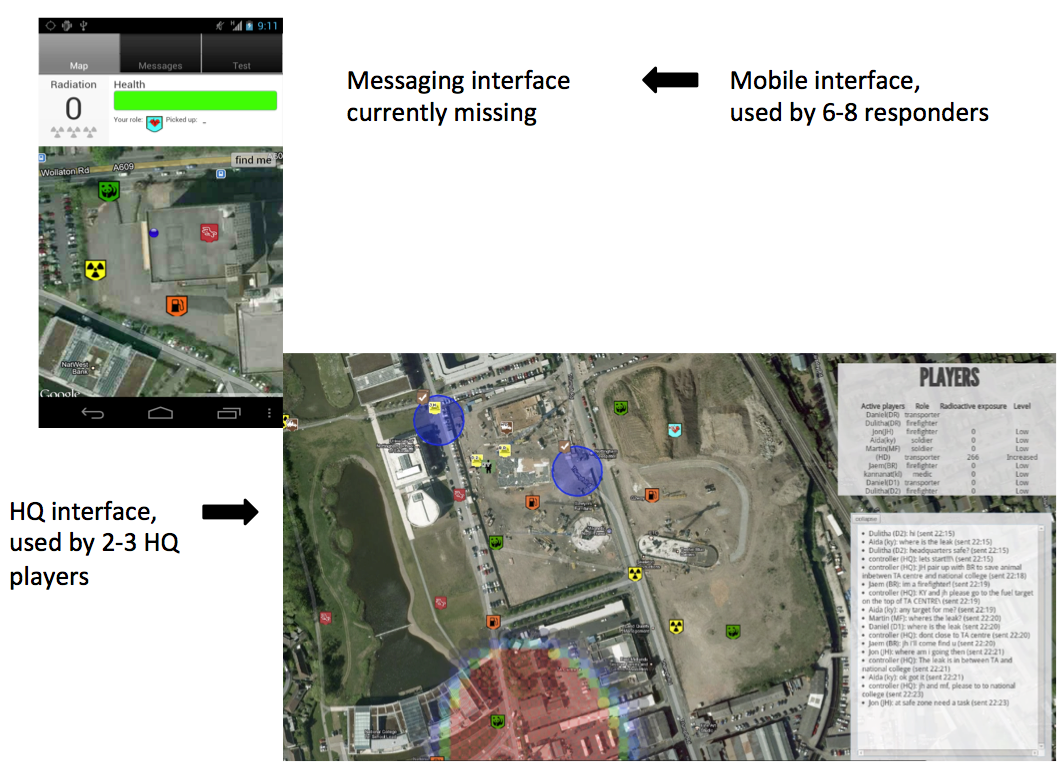
\includegraphics[width=1\textwidth]{img/conclusion/study1interface}
  \caption{Interface of study 1}
  \label{fig:study1interface}
\end{figure}



The 1st study discovered several flaws of the initial interface, which leads to a number of design requirements. 

\begin{enumerate}
	 \item The interface should support quick acknowledgement and feedback in communication channel.
	 \item The interface should freshness of messages in communication channel.
	 \item The interface should provide support for geo-reference.
\end{enumerate}

The second prototype is designed to integrate a planning support agent with an On-the-loop design pattern (Section \ref{sec:patterns}), in which HQ only monitors task allocation and execution with infrequent intervention. A set of changes in the second version (used in study 2) of AtomicOrchid are partly inspired by the requirements (see figure \ref{fig:study2interface}). In this version, all targets are identified by unique task IDs to support geo-referencing. Text messages in broadcasting channel are labelled by time stamp to flag potentially outdated information. With introduction of planning agent, the interface also supports quick feedback to the agent with one button press. With the integration of agent planning support, a new tab (``task'') in implemented in the mobile app to show a text-based description of agent task-assignment. In HQ interface, the agent assignments can be revealed on request of the HQ players (HQ clicking on "show task" button).\\

\begin{figure}[H]
  \centering
  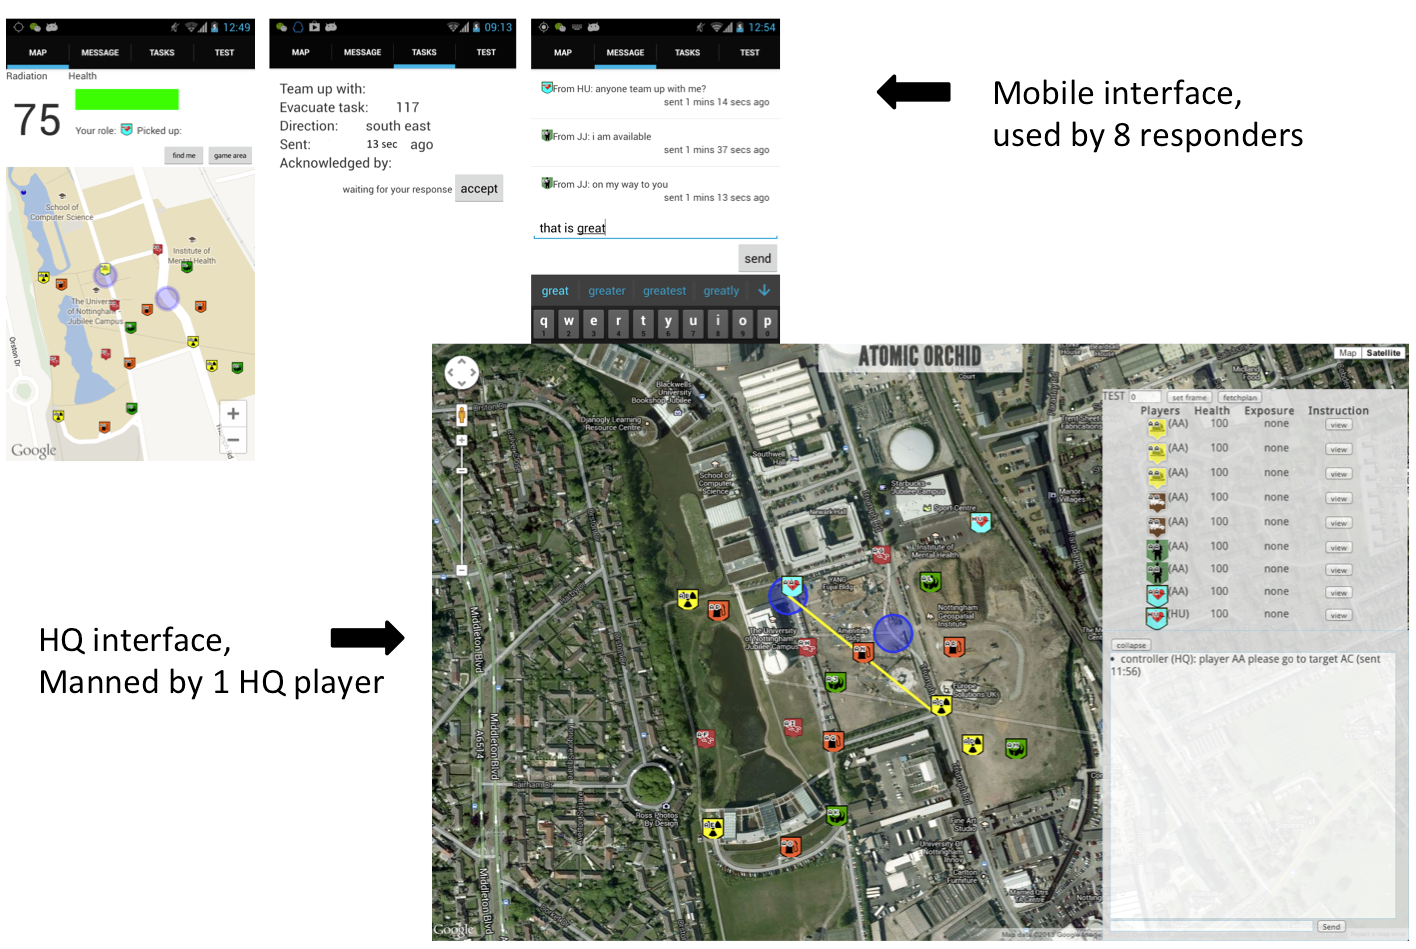
\includegraphics[width=1\textwidth]{img/conclusion/study2interface}
  \caption{Interface of study 2}
  \label{fig:study2interface}
\end{figure}

%purpose of the third study , lead to the interface. and requirements.
The result of the second study revealed that interface level support for HQ intervention is missing in the On-the-loop of AtomicOrchid. It is believed that the requirement for interface intervention support would also be important in the In-the-loop (the third) study. Therefore, a task assignment (see figure \ref{fig:study3interfacemobile}) interface are introduced to enhance the HQ's ability to intervene the task planning. A task-specific communication channel is also introduced in the interface for players to avoid information overload in broadcasting channel. Compared to previous HQ interfaces, the operations on the task assignment interface is a lot more complicated. Therefore, one HQ player is dedicated to operate the interface and another player is provided with On-the-loop version of HQ interface to provide situational awareness and handling broadcasting messages. 

\begin{figure}[H]
  \centering
  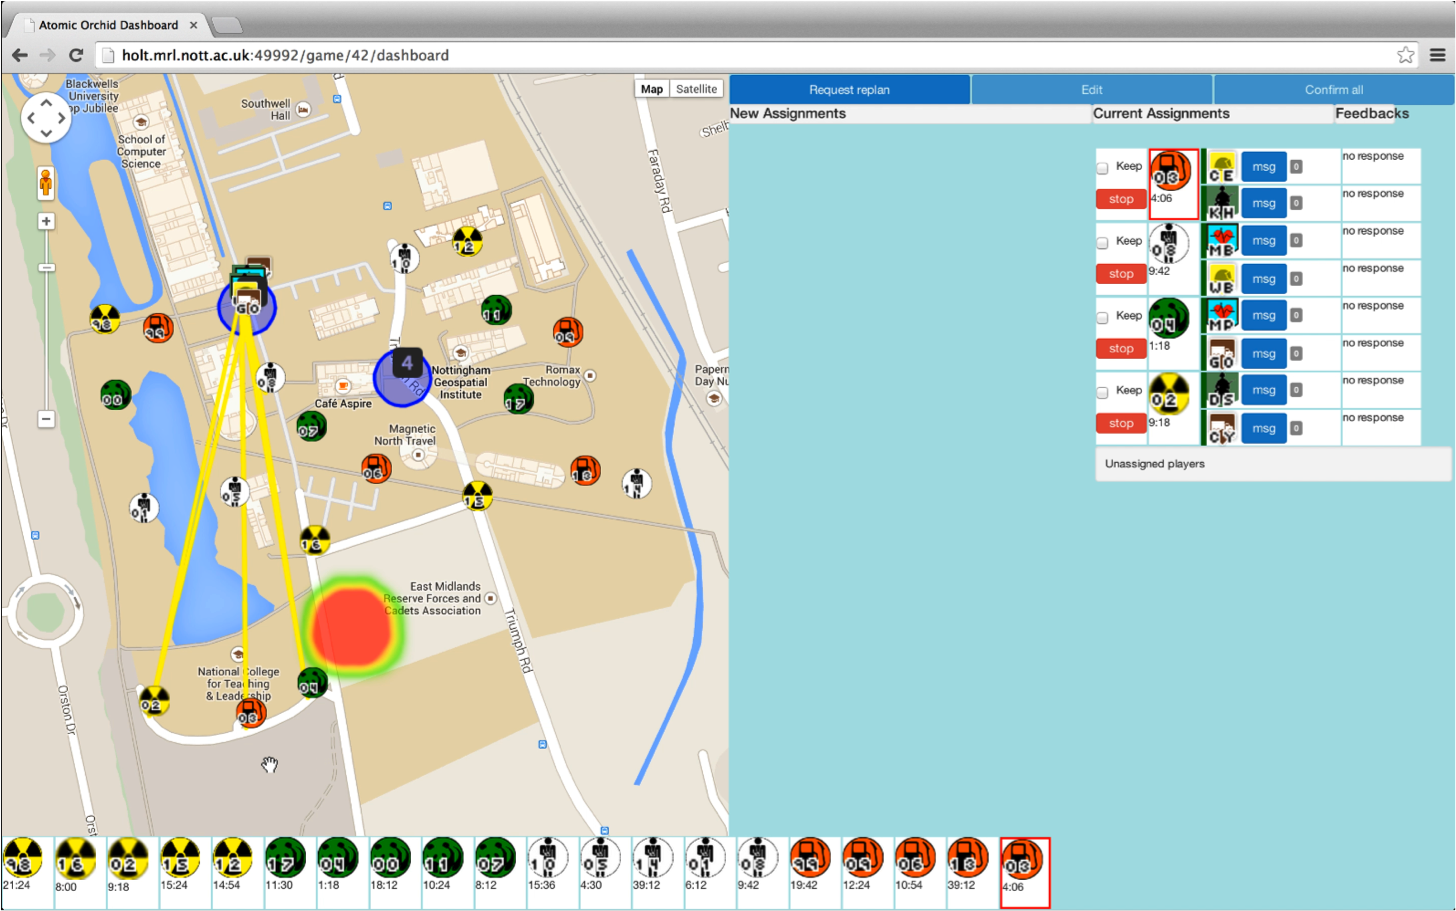
\includegraphics[width=1\textwidth]{img/conclusion/study3interfaceHQ}
  \caption{HQ Interface of study 3}
  \label{fig:study3interfacehq}
\end{figure}

For mobile interface, the tabs of ``status'' and ``chat'' kept unchanged from the version 2 (named ``map'' and ``messages''). The task interface is enhanced by a map-based presentation of task assignment and the task-specific chat box is displayed below the assignment (Figure \ref{fig:study3interfacemobile}.

\begin{figure}[H]
  \centering
  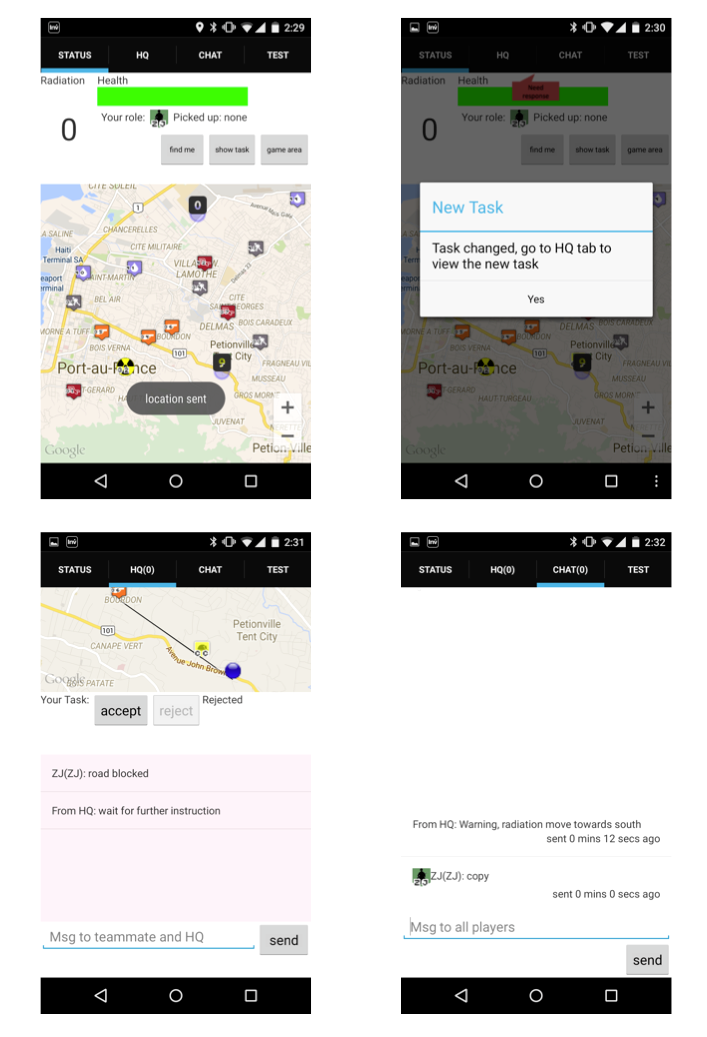
\includegraphics[width=1\textwidth]{img/conclusion/study3interfaceMobile}
  \caption{Mobile Interface of study 3}
  \label{fig:study3interfacemobile}
\end{figure}


\subsection{Key observations}\label{sec:conclusionOB}
This section gives a brief overview of the key observations from the three studies. First, the non-agent AtomicOrchid trial (study \ref{ch:studyone}) is aimed to give insight into how human conduct planning (without agent support) in the time and spatially constrained disaster settings and to generate general requirements of coordination support system which can be applicable to the next two agent-integrated versions of AtomicOrchid. The result of interaction analysis showed the team planning is dominated by local coordination between field players with in a ``situated'' manner. The field teams managed to organise their team and task allocations by utilising available resources such as local conversation, mobile interface, and remote messages. The HQ is observed to successfully provide awareness of the ``danger zone'' to the field teams through remote messages. However, HQ have little direct influences on the planning and actions of field teams. One potential reason could be the breakdown of communication between HQ and Field responders. The communication breakdown is thought to be caused by a set of factors including communication modalities (text vs voice), training level of players and HQ and system interface designs.  \\

In study 2, a planning agent is integrated to the system with the Human On-the-loop interaction design.  Through interaction analysis, we gain insight into the division of labour between human and agent (Section \ref{sec:studytwointroduction}) in which the agent takes over routine planning activities while the human focus on other issues such as finding teammates, targets and choosing the best routes. However, there are also evidence showing the agent planning occasionally interrupts workflow of human team potentially because it fails to consider social cost of task changes. We also observed HQ player struggled to influence the plan because the lack of interface level support. Further, a set of misconceptions in feedback loops (see section \ref{sec:studytwofeedback}) are also observed.\\

In study 3, the system is evolved to facilitate In-the-loop interaction with the feedback from study 2. The main changes are a number of interface functionalities which enable HQ to approve, edit agent planning and monitor player feedbacks. Through observing the usage of this new functionalities in the control room, we observed a pattern division of labour between in which:
% is it found or just desgin
	\begin{enumerate}
	 \item The HQ decide when to perform re-plan.
	 \item The HQ review every agent instruction for routine task planning.
	 \item The HQ deals with player feedback.
	 \item The Agent proposes task allocation.
	\end{enumerate}
	
Field observation shows this pattern of labour division is at least partially facilitated by the task assignment interface deployed in study 3 (Section \ref{sec:study3system}). The task assignment interface appears in many cases to provide an effective shared representation of the current state of the game. As well as showing current player and target locations and player health it also makes visible the currently approved task allocations, field player responses and any new plan that has been requested or is being edited. This shared information forms the common ground between the HQ players and the planning agent. HQ players are also observed to closely monitor this view and its representation of plan execution to gain awareness of cloud`s location in relation to players and current task progress. HQ players also engage actively with proposed (rather than current) task assignments. HQ players are quite capable of modifying the agent`s plans when they wish to, for better (Episode 3.3) or worse (Episode 3.4).\\

Analysis of some failed cases of coordination also points out a number of interactional issues. The details about the issues, possible solutions and design implications are discussed in the following section \ref{sec:conclusionIssue}. \\


\subsection{Interactional issues and lessons}\label{sec:conclusionIssue}
There are a number of interactional issues emerged from the field observations. This section reflects on interactional issues related to 4 themes including Division of labour, common ground, accountability and support of situated actions.

\subsubsection{Division of labour}\label{sec:conclusionHH}
The On-the-loop and In-the-loop interaction designs have been trialled in two studies. To recap, the main distinction between the two interaction design is the extent to which the human HQ is involved in routine task planning. For the On-the-loop design, the system is supposed to run without human input, while the In-the-loop system can not operate without constant human interaction. Guided by these two patterns, detailed system design has been implemented.\\

\begin{figure}[h]
  \centering
  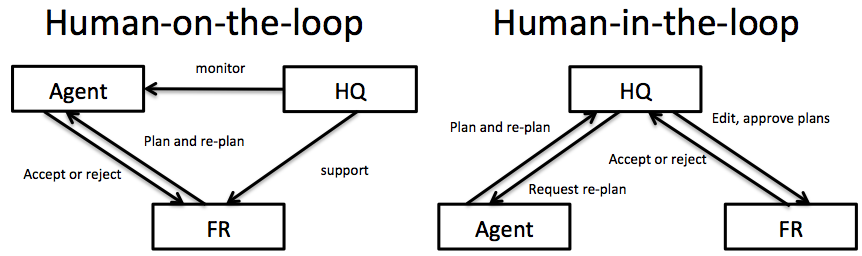
\includegraphics[width=1\textwidth]{img/conclusion/huilvshuol}
  \caption{On-the-loop vs In-the-loop}
  \label{fig:huilvshuol}
\end{figure}

\begin{table}[]
\centering
\tiny
\begin{tabular}{lllll}
Division of labour &  &  &  &  \\ \hline
 & FR & \begin{tabular}[c]{@{}l@{}}1. Interpret instructions\\ 2. Organise team meet-ups\\ 3. Deals with navigational issues \\ (Locate target, find routs)\\ 4. Provide feedbacks (accept/reject)\end{tabular} & \begin{tabular}[c]{@{}l@{}}1. Interpret instructions\\ 2. Organise team meet-ups\\ 3. Deals with navigational issues\\ (Locate target, find routs)\\ 4. Provide feedbacks (accept/reject)\end{tabular} &  \\ \hline
 & HQ & \begin{tabular}[c]{@{}l@{}}1. Monitor and chose to intervene\\ 2. Sending other information in\\ broadcast channel\end{tabular} & \begin{tabular}[c]{@{}l@{}}1. Initiate re-plan\\ 2. Review every agent instruction\\ (Edit when necessary)\\ 3. Send information in \\ broadcast channel\\ 4. Deal with feedbacks \\ from field responders\end{tabular} &  \\ \hline
 & Agent & \begin{tabular}[c]{@{}l@{}}1. Send task allocations directly\\  to field responders\\ 2. Initiate re-plan\\ 3. Deal with rejections \\ from field responders\end{tabular} & \begin{tabular}[c]{@{}l@{}}1. Send task allocations to HQ \\ for approval\\ 2. Perform partial task planning \\ based on constrians specified by HQ\end{tabular} &  \\
Interface support &  &  &  &  \\ \hline
 &  & \begin{tabular}[c]{@{}l@{}}1. Representation of game status\\ 2. Broadcasting message channel\end{tabular} & \begin{tabular}[c]{@{}l@{}}1. Representation of game status\\ 2. Broadcasting message channel\\ 3. Task-specific message channel\\ 4. Field responder feedback highlighting\\ 5. Support for plan edits\\ (Drag and Drop interface)\end{tabular} & 
\end{tabular}
\caption{On-the-loop vs In-the-loop}
\label{tab:onin}
\end{table}


There are several performance differences between the In-the-loop and On-the-loop studies. Direct comparison of performance between In-the-loop and On-the-loop is not applicable because the study 2 introduces a number of improved interface support (Figure \ref{fig:huilvshuol}) that influences team performance as well. However, the difference of performance can still leads to some implications of interaction design.\\

\begin{enumerate}
\item \textbf{In-the-loop design is an option to reduce unnecessary task interruptions} \\
As we have summarised in section \ref{sec:huilimperfection}, there are evidence showing that the On-the-loop design is more likely to cause extra re-teaming and task interruptions when compared to the In-the-loop design. In study 2, HQ has been observed to deliberately avoid unnecessary task interruptions and team reformations caused by agent planning. 

It can be argued that the difference is simply caused by lack of reliability of the agent. Some AI researchers have attempted to enhance the reliability of the planning agent in handling social situations (Section \ref{sec:lrinterfaceagent}) with the approach of a plan/intent recognition. For example, Some may believe planning agent with better user/environmental modelling techniques can factor in the social process involved in task changes to inform plan generation. However, the work of \cite{Suchman1987} has acknowledged the extreme difficulty of plan/intent recognition because of weak logical inferential connections between human's intents and actions in situ. Therefore, we believe that the In-the-loop design may be useful approach to overcome the agent's limited reliability and utilise its capability at the same time.\\

However, the In-the-loop design may also have its own cost. On one hand, it increases workload of HQ player because need to check each instruction proposed by agent. HQs sometimes failed to recognise task interruptions even with interface highlighting support, which suggest HQ can not help to eliminate all the unnecessary interruptions. Effectiveness of HQ may also depend on a balanced workload. In a multi-tasking control room environment, it is critical to balance the the workload of HQ. Therefore, we need to carefully consider the trade-off between the increase of workload and the reduction of unnecessary task-interruptions \\

\item \textbf{HQ's ability to intervene agent planning is required for both In-the-loop and On-the-loop design pattern.}\\
Compared to In-the-loop study, the HQ players in On-the-loop study are observed to struggle to intervene the planning process, and we believe the performance difference are at least partially linked to the distinction between In-the-loop and On-the-loop. In On-the-loop study, the only way for HQ to intervene the planning is to send unstructured text messages in broadcast channel. HQ's ability to intervene has been greatly enhanced by a set of interface support introduced in the In-the-loop study. Some of the interface support is inspired by the implications from On-the-loop study. It highlights the need of interface support for HQ intervention because both In-the-loop and On-the-loop requires HQ get involved when necessary. \\

\item \textbf{Human involvement may also incur system planning failure.} \\
Compared to On-the-loop design, the In-the-loop design supports greater human involvements in plan generation. However, some planning failure appears to be directly linked to human involvement in In-the-loop design. For example, there is a case of  human "death" occurred  when field players were trying to follow a human generated plan in the In-the-loop trial.  Although there are lots of factors contributing to the `death' case (e.g. insufficient training for field play, communication breakdown), the task assignment is thought to be too risky and not recommended by the agent at the first place. It is believed that the chance of human mistakes can be reduced by appropriate interaction design which helps to establish the `common ground' between human and agent. However, such a design would not be as easy task as it involves multiple design trade-offs  (Section \ref{sec:conclusionCG}).
\end{enumerate}

To sum up, the task interruptions are more frequent with the On-the-loop design (compared to the In-the-loop study). The fact highlights the lack of agents' ability to model the social process in human teams. Following the view of \cite{Suchman1987}, we believe human's intentions and actions in situ are extremely hard to be modelled. Thus, the In-the-loop interaction design maybe  a much more feasible approach to overcome the limited reliability of the agent, however, with expense of higher HQ workload. Secondly, the interface support for HQ intervention has been proved to be important in both In-the-loop and On-the-loop settings. Finally, a human involvement in planning (In-the-loop) are likely to incur some planning failure. The issue highlights the need for effective information sharing between human and agent, which help to establish the `common ground' for coordination. \\


\subsubsection{Establishing common ground} \label{sec:conclusionCG}
The ``Common Ground'' (or as \cite{Suchman1987} suggested ``mutual intelligibility'') is the basis for human agent interaction \cite{Bradshaw2011}.  While, the "common ground" maybe improved with plan/intent recognition technologies (e.g. user modelling), this approach, if possible, can be extremely difficult (Section \ref{sec:sociotech}). The author believe appropriate interaction design can enable human operators to understand and influence the planner agent. This section summaries the interaction design implications concerning the establish the  ``Common Ground''.\\

In both study 2 and 3, the agent behaves like a "black box" which gives the results (task allocation). The interface only exposes the results of agent for HQ to monitoring. Through our observations in chapter \ref{ch:studytwo}, \ref{ch:studythree}, we find there could be some extra information shared between human and agent to improve planning.\\

The HQ players is observed (section \ref{sec:study3discussion}) to occasionally make some forward planning for field players. Because the forward planning is also performed by the agent to derive current plan, the information could be shared so that the HQ players can be provided with the agent suggestion when doing forward planning.\\

The reasoning behind current task allocation would also be useful for sharing. In chapter \ref{ch:studythree} , HQ is found overriding agent plans, which leads to undesirable results. The HQ is also found being confused when agent stop assigning tasks to players with low health. Exposing internal reasoning of the agent can help the HQ to make informed decisions. \\

Misunderstanding between agent and human is also observed in the feedback loop in study \ref{ch:studytwo}. Firstly, human responders do not know how agent is going to handle the rejection. They try to use rejection to reverse back to previous tasks, while the agent will give them more new instructions. Secondly, it is unknown to field responders that their rejection will cause replanning for the whole team which can lead to lots of costly task interruptions. Therefore, information indicating consequence of interface interactions should be also made available to human to facilitate accountability and ensure informed decisions. \\

Although, we have identified a range of information which is missing for establishing "Common Ground", presenting the information could be also challenging. The information should be delivered in right form (e.g text, visualisation, dialogs) and in right time (e.g. pop up or on HQ request?) \cite{Carver2007} Especially in the multi-tasking, time-critical settings like AtomicOrchid, multiple sources of information can compete for attention of the human operator. Information overload could be a real danger of interaction design in this setting \cite{Lieberman2003}. Therefore, the  way for exposing agent's information and its human performance consequence may need to be further studied.   \\

\subsubsection{Faciliating accountability}\label{sec:conclusionAC}
The observation shows that both the spatial divide and the existence of the planning support can be the factors that affects natural accountability of member's activities. \\

In the 1st study, players heavily rely on local coordination for task planning. In a co-located setting, players can naturally make their actions observable and accountable to each other through conversations, body languages, gestures et al. In the distributed work setting, the spatial divide make accountability of member's activities opaque to each other. The technology support may need to play the role in supporting member's accountabilities. However, the reliance on local coordination indicates the lack of remote coordination support in the AtomicOrchid system. A set of functionalities including GPS/map sharing, broadcasting has been provided. We have observed players utilise the functionalities to make sense of other team members' actions (see section \ref{sec:s1localcoordination}) and act accordingly. However, coordination with remote players is still overall problematic which can be evidenced by frustrations related to remote communication (Section \ref{sec:study1breakdown}). Therefore, we suggest remote coordination support should be built in a way that facilitate accountability across the distributed team, by making player's activities observable and reportable.\\

In the 2ed study, The issues of members' accountability are further complicated by the existence of planning support. Individual player's interactions with the planner agent (reject/accept plans) have impact on the planning of the whole team. However, while the rules of social conduct ensured accountability of action among co-located teammates, we found the impact of rejections on remote players was not properly appreciated; nor did the interaction design support making these individual human-agent interactions accountable to the whole team. We believe the interaction design shall reveal the hidden cost of certain actions (e.g., rejections) to facilitate local decision making accountable to remote team members, ensuring consequences of local decisions for the welfare of all teams are understood. \\

\subsubsection{Supporting situated actions}\label{sec:conclusionSituatedAction}
The thesis takes the view of situated actions proposed by \cite{Suchman1987}. The problem solving agent necessarily produces plans in attempt to guide human teams, while human acts in a situated manner. There is a need to design interactions that bridge the gab between planning model of agent and situated actions of human. The observed human actions in studies is well aligned with the the view of situated actions. In the non-agent version of \ac{AO} players are able to organise their activities with all their available resources (local conversations, messages, game status from mobile interface) without reaching a ``plan'' for the whole team.  In the second (on-the-loop) study, players are observed to utilise the agent plans as an extra resources for taking action in various social situations (Section \ref{sec:study2social}). Based on our observations, we summaries some recommendations for supporting the situated actions. \\

\begin{enumerate}
\item \textbf{Presenting agent plans as a resource for situated actions.} The agent ``plan'' itself is a representation of actions and their projective effects \cite{Suchman1987}. One key task of system is to provide interface support for presenting the plans so that it can be easily utilised by human as a resource for deliberations on their actions. Through the three studies, we incrementally enhance plan representation. The final interface presents the agent plan in a structured way,  along side the the current task status (player feedbacks and existing plan under execution) and map-based location visualisation. This representation turns out to be effective for HQ players to make sense of the situation and act on the task allocation and monitoring.\\

\item \textbf{Facilitating the situated actions.} We observed that the human operators are faced with various social situations and contingent circumstance (Section \ref{sec:study2social}) in the field trials. The system may need to keep the flexibility to allow human to proceed with their actions, no matter whether they chose to follow the agent plan or not. With the On-the-loop version of \ac{AO}, the agent plans sometimes ``get in the way'' as hindrance rather then resources for players. The agent support system follows strict planning model (plan-act-replan) without sufficient support for human involvements. Consequently, although he human can chose to ``disobey'' agent (by rejecting, or ignore), the result is the complete abandon of the use of the agent or even more problematic confusions (e.g. Episode 2.4 in Section \ref{sec:study2analysis}). On the other hand, the In-the-loop version of interface facilitates the flexibility for human actions by providing interface functionalities for plan edits and opportunity moment in the workflow for intervention. In this way, frequent human inputs are synthesized with the agent plan as a resource that support their situated actions. \\

\item \textbf{Supporting human-system mutual intelligibility.} By adopting the view of human agent interaction (Section \ref{sec:LRHAI}), the support system can be treated as equal team player, with whom the mutual intelligibility should also be maintained to achieve concerted action \cite{Suchman1987}. Here we treat the Mutual Intelligent and Common Ground are interchangeable concepts.  Therefore we can refer to section \ref{sec:conclusionCG} for suggestions on improving mutual intelligibility. \\
\end{enumerate}

%Mutual intelligibility is originally used to describe shared understanding in human teams, which is essential for concerted actions. In the context of AtomicOrchid, the existence of system should not hinder but support the achievement of mutual intelligibility among human team members. In the study 2 particularly , we found there is a danger to block natural human accountability in the human teams (Section x) as a result of failure to support  . 

\section{Limitation}
This section outlines some of the limitations of this PhD work. \\

By following a serious mixed reality game approach, the game AtomicOrchid is used to simulate some key factors of the distributed, time-critical task setting.  The fictitious game scenario can not completely mirror the setting of disaster operations. Firstly, the time-scale of planing is match longer in a rescue and reconnaissance mission (from hours up to days, Section \ref{sec:RGworkshopone}), while the AtomicOrchid only have 30 mins time-scale. Secondly, the disaster response teams always priorities critical tasks according to some specific code of conduct (e.g. task with human injuries will always be prioritised.). Therefore, the game objective of maximising targets saved may not match real goal of DR team. According to professional feedbacks (\ref{sec:RGworkshopone}), the communication modality (text, rather then radio) and the assumption `constant connectivity' is also not aligned with real world response task. \\

Further, the seriousness of the simulation can also be a limitation of game approach. Participants are frequently observed to laugh and make jokes about their health values (life), which indicates they take the trials as a recreational experience. Therefore, the participants maybe less concerned about risk and life threats, when compared to real disaster setting. \\

The untrained participants are recruited for the field trials. We anticipate that the behaviours of players in the game may change with their training experience. Further, the professional responders can also behave differently because they have high level of training, real experience of \ac{DR} operations, different code of conduct and organisation structure.\\

In terms of data analysis, the result may not have quantitative robustness because we only 6 game trials are conducted. This limitation is actually a limitation of the data analysis method we apply, namely interaction analysis. The method is extremely time consuming, thus limiting the number of data we can analysis \cite{Crabtree2012}. With limited trials and participants, the individual difference (of participants and teams) can significantly affects the generality of the study results. Consequently, the generality of the results may have to be established with other means. However, this limitation does not affects the descriptive power of qualitative approach of the analysis. \\

Overall, the PhD work employed a game approach, which has a number limitations in terms of game scenario participants' altitude, participants' selection and data analysis method. We can not claim the observations of human behaviours based on game approach would be exactly the same as what happens in the real disasters. However, we argue that the game-based approach can introduce some critical factors of \ac{DR} operations, including time pressure, distributed team setting, and the mental/physical stress. Compared to computational simulation, the field trials can reveal rich human-system interactions under time and spatially constrained task environment. Therefore, we argue the observations from game trials are still valid and can be used to generate design implications for future \ac{HACS} systems. \\


\section{future work}
Following the limitations and contributions of the thesis, its impact can be extended into future work in several possible ways. Firstly, the planning agent itself might be improved with various AI technologies. For example, the agent in this study does not consider the social cost of re-teaming and task interruption. For example, we can explore other AI technologies such as user modelling techniques (Section \ref{sec:lraisupport}) to model the human social behaviour and factor it in to the plan generation process.  However, when agent is enhanced by new AI technologies, it is unknown whether the new capabilities would hinder or improve team coordination and how the interaction design should be adapted to support the new capabilities. Therefore, one future direction of this PhD study is to incrementally enhance agent capabilities and conduct observational studies to gain insight into the implications of the new enhancement on the interaction design.\\

Secondly, the game can be re-engineered so that the game setting can be better grounded in the real practices of disaster operation team. In order to do that, the close collaboration with disaster response teams may be required. The collaboration with Global Rescue happened in the late stage of this this PhD work, which help us to identify some potential improvement of the game setting. Firstly, the targets are not always equally important. For example, human injury will typically be prioritised. Considering different weighting on targets can make the game setting more realistic. Secondly, radio rather then text messages is the communication modality used by operation teams, which may have impact on our behaviour observations. Thirdly, the AtomicOrchid assume constant connectivity between HQ and field responders, but the disaster operations are often characterised by intermittent communication. Therefore, it would also be useful to simulate the intermittent communication in AtomicOrchid.  \\

In a similar vein, the subjects of study might be changed to professional responders in order to better elucidate human behaviour in real disaster operation.  As we believe that the trained professional responders may behave differently with the general public. It would be desirable to recruit professionals in the future work to validate the findings of this PhD study.\\

In terms of the methodology, more field trials might be conducted in order to carry out statistically robust quantitative analysis. If there are more field trials, quantitative analysis can compliment the qualitative interaction analysis in some aspects. For example, the statistical difference in terms of games results (including players death, targets saved) can be used to imply effectiveness of interaction designs. Also, the social cost and workload of HQ may also be quantified  to give insight into the impact of interaction designs on the team performance. \\ %cognitive modelling of workload.

The studies have highlighted the trade-off between establishing common ground and information overload (Section \ref{sec:study3discussion}). It is believed that further studies can focus on answering how the trade-off affects team coordination and develop guideline for system designer to balance trade-off. \\  

Moreover, the interaction designs are not limited to the On-the-loop and In-the-loop. Contribution of this PhD work can be extended by exploring some middle-ground designs. For example, the agent can be given the responsibility to decide when to perform a re-plan (as it is in the On-the-loop design), but also send the instructions to HQ for approval (as it is in the In-the-loop design).\\

It should also be noted that the centralised planning support is only one kind of agent planning support technology among many. For example, the planning support can also be decentralised. The planning agents can be built into personal assistant devices for every field responders. We believe that The change of agent technologies have implications on interaction design. New interaction design pattern can be devised and adopted with the change of agent technologies. Therefore, this PhD work can potentially be extended with exploration of different automated planning support technologies.\\ 

Further, this work contributes to the research paradigm of \ac{HACS} system (Section \ref{sec:lraisupport}) by studying the interaction between one centralized planning agent and a disaster response team. However, the \ac{HACS} researchers envision a scenario in which large amount of computational entities (including both software agents and embodied agents such as rescue robots ) and human teams collaborate at large scale. For future work, there is a potential to extend AtomicOrchid incorporate multiple agents and human teams to study multi-agents and human interaction.\\




